\documentclass[a4paper,11pt]{article}

\usepackage[spanish]{babel}
\usepackage[utf8]{inputenc}
\usepackage{hyperref}
\usepackage{graphicx}
\usepackage{amsmath}
\graphicspath{{images/}} 

\author{Daniel Monjas Miguélez}
\title{FR: Tema 2}

\begin{document}
\begin{titlepage}
\centering
    \vfill
    {\bfseries\Large
        Fundamentos de Bases de Datos: Tema 2\\
        28 de Noviembre del 2020\\
        A year to Forget \\
        \vskip2cm
        Daniel Monjas Miguélez\\
    }    
    \vfill
    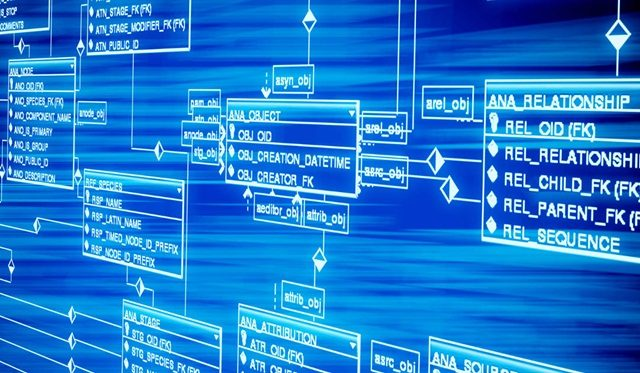
\includegraphics[width=13cm]{bases_datos.jpg}
    \vfill
    \vfill
\end{titlepage}

\newpage
\tableofcontents
\newpage

\section{Niveles generales de la arquitectura:}
¿Por qué organizar en niveles?

\begin{itemize}
\item Los usuarios pueden acceder a los mismo datos, pero desde distintas perspectivas. Si un usuario cambia la forma de ver los datos no influye en el resto.

\item La organización global de los datos puede cambiarse sin afectar a los usuarios.

\item Los usuarios no tienen por qué gestionar aspectos relativos a la presentación física de los datos. El administrador de la base de datos puede cambiar la forma de representar los datos sin influir en los usuarios.
\end{itemize}

\textbf{Arquitectura ANSI/SPARC}: La percepción de los datos de un Sistema Gestor de Base de Datos puede hacerse siguiendo tres niveles de abstracción (nivel interno, nivel conceptual y nivel externo). Su predecesor es el modelo CODASYL-DBTG, el cual tenía solo dos niveles. \\

\textbf{Los tres niveles:}
\begin{itemize}
\item \textbf{Nivel Externo:} en este se definen las distintas percepciones particulares de la base de datos por parte de los usuarios (Vistas de Usuario). Excluye datos irrelevantes, así como los datos que el usuario no está autorizado a acceder.

\item \textbf{Nivel Conceptual:} abstracción global de la base de datos. Integra todas las percepciones que los distintos usuarios tienen de la base de datos. Este nivel solo puede ser definido por el Administrador de la Base de Datos y es independiente de hardware y software.

\item \textbf{Nivel Interno:} representación de la base de datos más cercana a la estructura de almacenamiento físico. Estructuras de datos sobres las que se sustentan los niveles superiores. En él se describe cómo los datos se almacenan en la base de datos y en el hardware del equipo. En este nivel también trabaja el Administrador de la Base de Datos.
\end{itemize}

\begin{figure}[h]
\centering
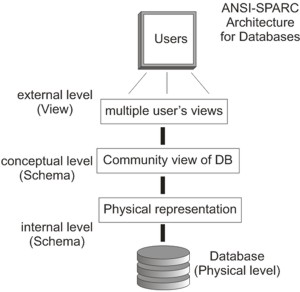
\includegraphics[scale=1, width=0.9\textwidth]{esquema_niveles.jpg}
\end{figure}

\textbf{Correspondencia o correspondencia entre niveles:} Son el conjunto de normas que establece cómo se definen los datos de un nivel en términos de otros. Es un mecanismo fundamental para el establecimiento de independencia, bien sea lógica o física.

\begin{itemize}
\item \textbf{Transformación conceptual/interna:} cómo se organizan las entidades lógicas del nivel conceptual en términos de registros y campos almacenados en el nivel interno. Preserva la independencia física. Es implementada por el Sistema Gestor de Bases de Datos. Son aspectos gestionados por el Administrador de la Base de Datos (índices y clusters). Si varía el nivel interno cambia la correspondencia pero no varía el nivel conceptual.

\item \textbf{Transformación externa/conceptual:} describe un esquema externo en términos del esquema conceptual subyacente.Preserva la independencia lógica. El Sistema Gestor de la Base de Datos determina la forma en que se implementan y almacenan y el DSL (Domain Specific Languages) permite definirlas. Algunos SGBD permiten definir el nivel interno en función del SO, usualmente de forma transparente. Permite portabilidad. Si varía el nivel conceptual, cambia la correspondencia pero no varía el nivel externo. No siempre es posible este tipo de transformación.

\item \textbf{Transformación externa/externa:} algunos SGBD permiten describir esquemas externos en términos de otros esquemas externo. Preserva la independencia lógica. Si varía el esquema externo subyacente cambia la correspondencia pero no varía el esquema definido. Al igual que el anterior no siempre es posible.
\end{itemize}

\begin{figure}
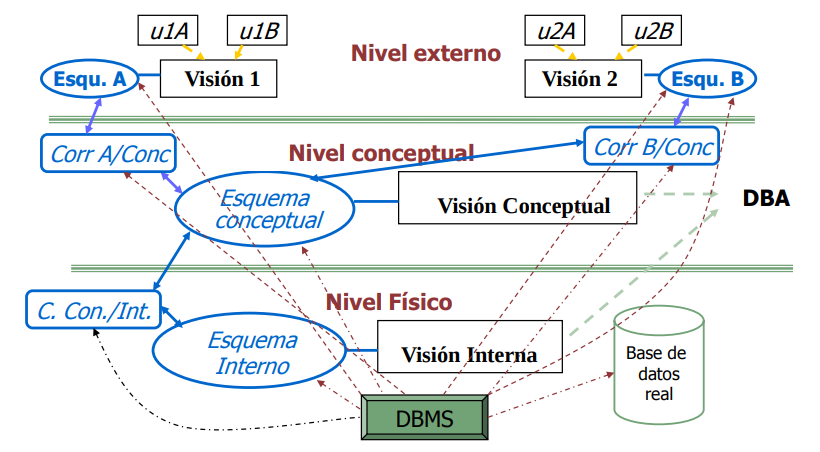
\includegraphics[scale=0.7]{correspondencia_niveles.png}
\caption{Esquema de transformación entre niveles}
\end{figure}

\textbf{Lenguajes de un BD:} La recomendación para la arquitectuaras ANSI/SPARC es disponer de un lenguaje específico orientado a los datos, y que permita la definición, el control y la manipulación de los mismos. \\

\textbf{DSL (Domain Specific Language)}: es implementado en el propio SGBD. Este dispone de distintas partes DDL(Data Definition Language), DML (Data Manipulation Language), DCL (Data Control Language) y Lenguajes anfitrión (Host Language).

\begin{itemize}
\item \textbf{Data Definition Language (DDL):} es un subconjunto del DSL para definición de estructuras de datos y esquemas de la BD.

\item \textbf{Data Manipulation Language (DML):} es un subconjunto del DSL para introducción de datos, modificación de datos, eliminación de datos y consulta de datos. También debe permitir consultar los esquemas definidos en la BD.

\item \textbf{Data Control Language (DCL):} es un subconjunto del DSL para gestionar los requisitos de acceso a los datos y otras tareas de administración de la BD.

\item \textbf{Lenguaje anfitrión (Host Language):} lenguaje de aplicación de alto nivel que incluye al DSL como una ampliación.
\end{itemize}

La arquitectura ANSI/SPARC recomienda disponer de un DDL, un DML y un DCL para cada nivel de la arquitectura. En la práctica todos estos sublenguajes se presentan bajo una implementación única. Aunque las sentencia son distinguibles a nivel de categoría la separación de los lenguajes conforme a los niveles de la arquitectura se establece de acuerdo con el tipo de sentencia que puede ejecutar cada usuario según privilegios. Cada sentencia trabaja sobre uno o varios niveles. Un sistema de privilegios se encarga de discriminar quién puede ejecutar qué. Por otro lado la insdustria ha seguido un camino diferente, el de los lenguajes de datos estándares. \\

Lenguaje anfitrión o de aplicación. Es un lenguaje para desarrollo de aplicaciones en el SO que trabajen sobre la BD. Son lenguajes de propósito general (C/C++, Java, C\#...), herramientas de desarrollo específicas (Developer de Oracle, Oracle Application Express (Oracle APEX), Sybase PowerBuilder, IBM Rational Application Developer,...), y proporcionan un procesamiento avanzado de datos y una gestión de la interfaz de usuario. Hay que establecer un mecanismo para traducir estructuras de datos y operaciones. Además debemos distinguir en cuanto al acoplamiento del lenguaje:

\begin{itemize}
\item Debilmente Acoplados. Son lenguajes de propósito general. El programador puede distinguir sentencias propias del lenguaje anfitrión de sentencias dispuestas para acceder a la BD a través del DSL. Se dota al lenguaje de prop.(¿?) general de mecanismos para interactuar con el DSL de la BD. Implementación mediantes APIs de acceso a BD: ODBC (Open Database Connectivity), JDBC (Java Database Connectivity) y DSL Inmerso en el código fuente del lenguaje anfitrión (El programador escribe un código híbrido que mezcla sentencias del lenguaje anfitrión con sentencias DSL. Un preprocesador luego lo transforma. Ejemplo SQL inmerso en C, SQLJ...).

\item Fuertemente Acoplados.Son lenguajes y herramientas de propósito específico. Se parte del DSL como elemento central y se le incorporan características procedimentales (estructuras de control, entrada/salida o interfaz) para facilitar el desarrollo de aplicaciones. Implementación mediante PL/SQL de Oracle (Extensión Procedural para SQL) o ejecución de Java sobre una máquina virtual implantada en el propio SGBD.
\end{itemize}

También han aparecido numerosos entornos de desarrollo específicos para el desarrollo de aplicaciones de gestión (diseñadores de informes, diseñadores de formularios, ...).

\section{Nivel Externo}
Se trata de la parte de la BD que es relevante para cada usuario. Un usuario solo tiene acceso a aquellas entidades, relaciones y atributos que le son de interés. Estas están representadas de la forma que le interesa al usuario (Nombre completo o nombre y apellidos, fecha o día,mes y año...). También son datos calculados a partir de los que hay (edad, ventas totales,...).

\section{Nivel Conceptual}
En este nivel tenemos una visión global de los datos. Se trata de la estructura lógica de los datos, qué datos están almacenados y qué relaciones hay entre ellos. Este nivel representa todas las entidades, atributo y relaciones, las restricciones que afecta a los datos, la información semántica sobre los datos y información de seguridad y de integridad. También da soporte a cada vista externa y no debe contener ningún detalle de almacenamiento.

\section{Nivel Interno}
Se trata de la representación física de la BD en el ordenador y cómo están almacenados los datos. Este nivel busca el rendimiento óptimo del sistema y representa estructuras de datos, organizaciones en ficheros, comunicación con el SO para gestionar el uso de unidades de almacenamiento y compresión de datos, cifrado.... Parte de las responsibilidades de este nivel las realiza el SO y parte el nivel físico. No existe una división clara, depende de cada SGBD y de cada SO.

\section{Administrador de la BD}
La figura del DBA es de primordial relevancia en el contexto de los SGBDs. Entre las funciones del DBA se encuentran:

\begin{enumerate}
\item Definir el esquema conceptual, analizar las necesidades de información de la empresa, identificar los datos operativos, elaborar el esquema lógico e implantar el esquema conceptual.

\item Deciden la estructura de almacenamiento en el nivel interno, tanto el esquema interno como la correspondencia conceptual/interna asociada.

\item Establecen conexión con los usuarios, analizan los requerimentos, realizan diseño lógico y la codificación del esquema externo y las correspondencias externa/conceptual.

\item Definen las restricciones de integridad, establecen reglas (genéricas (independientes de la semántica del problema) y específicas(reglas de negocio)) e incluyen si es posible la integridad en el esquema conceptual.

\item Definen e implantan la política de seguridad, tanto de gestión de usuarios (determinar quienes acceden) como de privilegios (con qué nivel de acceso se accede).

\item Definen e implantan la estrategia de recuperación frente a fallos. Los SOs y los SGBDs suelen incorporar facilidades para afrontar los fallos, por ejemplo SGBDs redundantes o los RAID (Redundant Array of Inexpensive Disks). El DBA puede y debe realizar copias de seguridad de la BD y se encarga de las políticas de gestión de transacciones. Además incluye estrategias de relanzamiento para evitar estados inconsistentes.

\item También se encargan de la optimización del rendimiento. Tareas como liberar espacio no utilizado, determinar la necesidad de nuevos recursos hardware (gestión del nivel interno), reorganizar las operaciones para que se ejecuten de forma más rápida y establecer prioridades en el uso de los recursos (gestión de prioridades de consultas).

\item Además se encargan de monitorizar el SGBD, realizando un seguimiento continuo de la actividad del sistema, con tareas como auditar el acceso de los usuarios a los diversos recursos de la BD, comprobar los niveles de uso de los sistemas de almacenamiento y evaluar la eficiencia con que se realizan las operaciones.
\end{enumerate}

\section{Tipos de arquitecturas de implantación}
El concepto de SGBD ha evolucionado bastante, paralelamente al desarrollo de la informática, actualizando la forma de gestionar información, ejecutar los programas y de interactuar con el usuario.  \\

Inicialmente se tenía un esquema centralizado, donde toda la carga de gestión y procesamiento de información reacía en servidores centrales, a los que el usuario accedía mediante terminales. En el ordenador principal se hallaban el SGBD y los programas de aplicación. 

\begin{figure}[h]
\centering
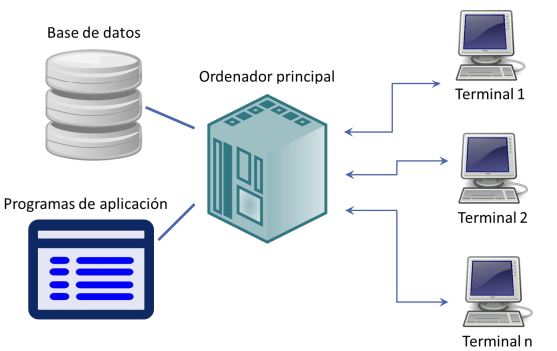
\includegraphics[scale=1,width=0.8\textwidth]{arquitectura_centralizada.png}
\caption{Esquema de arquitectura centralizada.}
\end{figure}

El problema era que el coste de los ordenadores principales era muy elevado (aparece el PC). La solución fue desplazar la ejecución de los programas de usuario y la interacción hasta los PCs, reduciendo así costes en hardware. Se hace una aproximación Cliente/Servidor, donde el servidor es el servidor de la BD y escucha peticiones. Los PCs están conectados en red con el servidor y ejecutan de programas de aplicación. Para la comunicación, el servicio de enlace del cliente interactúa con el servicio de escucha del servidor.  El desarrollo de las redes de comunicaciones se da mediante un enfoque distribuido.

\begin{figure}
\centering
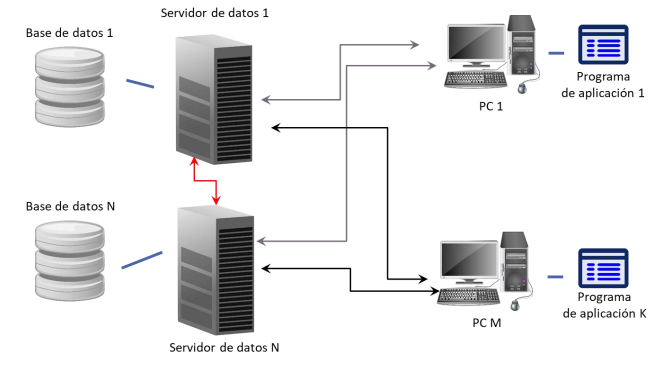
\includegraphics[scale=0.9]{arquitectura_distribuido.png}
\caption{Esquema de arquitectura distribuida}
\end{figure}

El problema de la aproximación cliente servidor es el alto coste de mantenimiento de los PCs (instalación, configuración y actualización). La solución fue separar en las aplicaciones las partes que interactúan con el usuario (interfaz) y las oartes de ejecución lógica del programa. \\

Actualmente se utiliza normalmente una arquitectura articulada en tres niveles de procesamiento.
\begin{itemize}
\item \textbf{Nivel de servidor de datos:} posiblemente distribuido. El SGBD permite organizar la información de la empresa como una BD global, donde las peticiones de datos formuladas desde una sede se traducen de forma transparente a peticiones en las sedes donde se encuentran esos datos.

\item \textbf{Nivel de servidor de aplicaciones:} Son evoluciones de Servidores Web que proporcionan los programas de aplicación a Clientes ligeros, que disponen de entornos de ejecución de aplicaciones, usando estándares, protocolos de red TCP/IP, protocolo HTTP, despliegue de Applets Java a ejecutar en Navegadores con soporte de máquina virtual Java y Servlets, JSP (JavaServer Pages), ASP, etc.

\item \textbf{Nivel de Cliente:} PCs ligeros dotados de configuraciones basadas en estándares abiertos. En muchos casos se pueden ejecutar las aplicaciones desplegadas en un navegador web con soporte de ejecución de código javascript y html avanzado. Basados en el carácter portable con que se distribuyen las aplicaciones desde los servidores de aplicaciones. Proporciona menos dependencia del hardware y del SO a la hora de abordar la ejecución de aplicaciones.
\end{itemize}

\begin{figure}
\centering
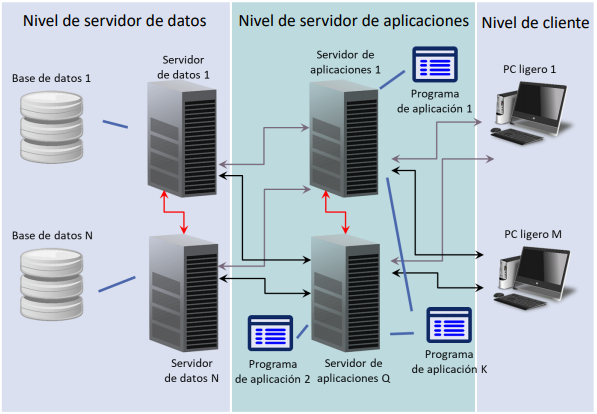
\includegraphics[scale=1,width=0.8\textwidth]{arquitectura_tres_capas.png}
\caption{BD distribuida y programas de aplicación en arquitectura de tres capas}
\end{figure}

Como ventajas está una reducción significativa en cuanto al mantenimiento de los clientes (instalación, configuración y actualización de las aplicaciones realizada en el servidor, no en cada cliente) y una mayor facilidad y flexibilidad para el usuario, que puede acceder desde casi cualquier puesto y desde distintos dispositivos: móviles, tables, portátiles, pcs, etc. \\

Como inconvenientes encontramos una mayor complejidad en la configuración y administración de los servidores de aplicaciones y el desarrollo de aplicaciones conforme a este modelo distribuido.

\section{Glosario}
\begin{itemize}
\item \textbf{Servlet}: es una clase en el lenguaje de programación java, utilizada para ampliar las capacidades de un servidor.
\end{itemize}
\end{document}